\documentclass[14pt]{extarticle}
\usepackage{fontspec}
\usepackage{polyglossia} % use instead of babel
\usepackage{pgfplots}
\usepackage{float}
\usepackage{amsmath}
\setdefaultlanguage{hebrew}
\setotherlanguage{english}
\newfontfamily\hebrewfont[Script=Hebrew]{Arial}

% TODO: figure out if better to keep this or not, for word document pdf output similarity
\usepackage[margin=1in]{geometry}

% might be useful to ensure similarity to word document pdf output
% \usepackage{setspace}
% \singlespacing

% Reset equation counter at the start of each section
\usepackage{chngcntr}
\usepackage{etoolbox}
\counterwithin*{equation}{section}
\preto{\section}{\setcounter{equation}{0}}


\begin{document}

\begin{center}
    {\LARGE \textbf{ממ"ן 12}}\\
    {\textbf{אופטיקה גיאומטרית}}
\end{center}

\begin{itemize}
    \item מגישים: תומר רוזנלפלד, שי רואימי
    \item תאריך ביצוע הניסוי: 19 יולי 2025
    \item מדריך הניסוי: ד"ר סילביו ריינהורן
\end{itemize}

\section*{ניסוי 1 - חוק סנל}
\subsection*{מטרת הניסוי}
מציאת מקדם השבירה של פקספקס 

\subsection*{רקע תיאורטי}
במעבר אור מתווך חומר אחד לאחר, זווית השבירה תלויה במקדם השבירה של שני החומרים, ובזווית הפגיעה.
חוק סנל מתאר את הקשר בין זוויות השבירה והכניסה של האור בחומרים שונים.
מקדם שבירה מוגדר בנוסחא:

\begin{equation}
    n = \frac{c}{v}
\end{equation}

כאשר $c$ היא מהירות האור בריק ו-$v$ היא מהירות האור בחומר.


חוק סנל קובע את הקשר בין זוויות השבירה והכניסה של האור בחומרים שונים:

\begin{equation}
n_1 \sin(\theta_1) = n_2 \sin(\theta_2)
\end{equation}

כאשר $n_1$ ו-$n_2$ הם מקדמי השבירה של החומרים 1 ו-2, ו-$\theta_1$ ו-$\theta_2$ הן זוויות הפגיעה והשבירה בהתאמה.

\subsection*{מערכת המדידה ומהלך הניסוי}

כיוונו קרן אור כלפי חצי דסקה עשויה פרספקס, ובעזרת מד זווית מדדנו את זוויות השבירה בהנתן זוויות פגיעה שונות. בעזרת תוצאות המדידה מצאנו את מקדם השבירה של הפרספקס.

הניסוי נעשה בעזרת מנסרה חצי עגולה. צורה זו משרתת את הניסוי בכך שכאשר קרן האור יוצאת מהמנסרה אינה "נשברת", כי זווית הפגיעה תמיד 0 מעלות, כי רדיוס במעגל ניצב תמיד למשיק למעגל בנקודת ההשקה.

\subsection*{תוצאות הניסוי וניתוח התוצאות}

מדידת זווית השבירה בהינתן זווית פגיעה שונה, הובילה לתוצאות הבאות:
\begin{center}
    {\normalsize
    \begin{tabular}{|c|c|c|c|}
    \hline
    זווית פגיעה (מעלות) & זווית שבירה (מעלות) & סינוס זווית פגיעה & סינוס זווית שבירה \\ \hline
    10 & 7   & 0.1736 & 0.1219 \\ \hline
    20 & 13.5 & 0.3420 & 0.2334 \\ \hline
    30 & 20  & 0.5000 & 0.3420 \\ \hline
    40 & 26  & 0.6428 & 0.4384 \\ \hline
    50 & 31  & 0.7660 & 0.5150 \\ \hline
    60 & 36  & 0.8660 & 0.5878 \\ \hline
    70 & 40  & 0.9397 & 0.6428 \\ \hline
    80 & 43  & 0.9848 & 0.6820 \\ \hline
    \end{tabular}
    }
\end{center}

\begin{figure}[ht]
  \centering
  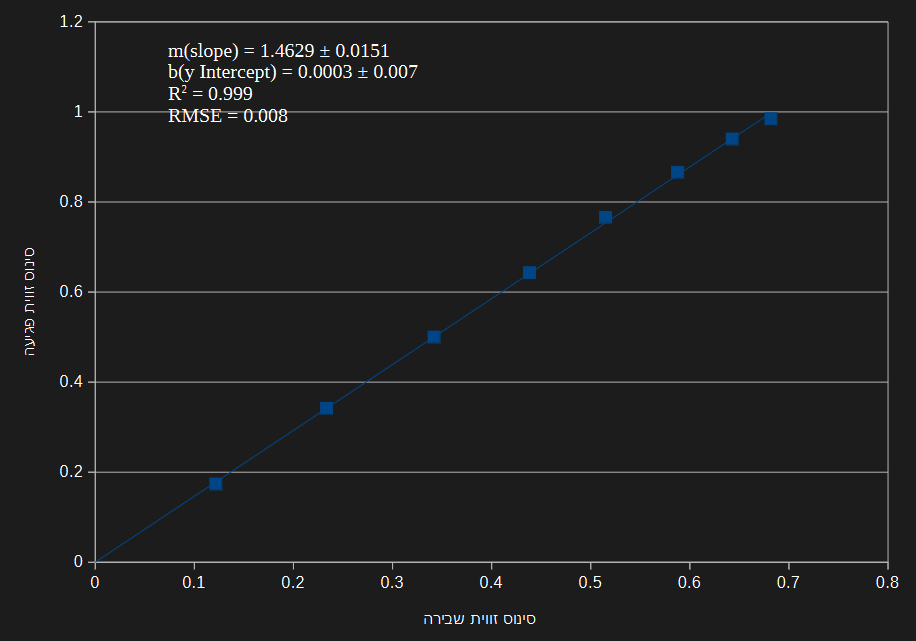
\includegraphics[width=0.8\textwidth]{Lab_1_Experiment_1.png}
  \caption{גרף המתאר את סינוס זווית הפגיעה כתלות בסינוס זווית השבירה}
  \label{fig:excel_chart}
\end{figure}

על מנת למצוא את מקדם השבירה נעזר בנוסחא:
\begin{equation}
n_{perspex} = \frac{n_{air} * \sin(\theta_1)}{\sin(\theta_2)}
\end{equation}
כאשר $n_{air}$ הוא מקדם השבירה של האוויר ($n_{air}=1$), $\theta_1$ היא זווית הפגיעה ו-$\theta_2$ היא זווית השבירה. נקבל:
\begin{equation}
n_{perspex} = \frac{\sin(\theta_1)}{\sin(\theta_2)}
\end{equation}

נצייר את הנקודות שהתקבלו במדידות בגרף, קיבלנו גרף ליניארי כאשר שיפוע הגרף הוא מקדם השבירה של הפרספקס. קיבלנו את הערך 1.46.

\subsection*{דיון ומסקנות}
הניסוי הצליח להדגים את חוק סנל ואת הקשר בין זוויות השבירה והכניסה של האור בחומרים שונים.

הערך הידוע בספרות הוא  1.49 (אתר אינטרנט - ,(https://refractiveindex.info השגיאה היחסית היא 2.02\%, וככל הנראה נובעת מ:
\begin{itemize}
    \item שגיאת המדידה של מד הזווית היא 0.5 מעלות
    \item רוחב קרן האור
    \item דיוק בתהליך המדידה
\end{itemize}

\section*{ניסוי 2 - החזרה גמורה}
\subsection*{מטרת הניסוי}
מציאת מקדם השבירה של פרספקס באמצעות מציאת הזווית הקריטית

\subsection*{רקע תיאורטי}
כאשר קרן אור פוגעת בחומר בעל מקדם שבירה גבוה יותר, היא נשברת בזווית מסוימת. כאשר זווית זו עולה על זווית מסוימת, הקרן אינה נשברת אלא מוחזרת לחלוטין. זווית זו נקראת הזווית הקריטית.

\subsection*{מערכת המדידה ומהלך הניסוי}

הפעם נהפוך את חצי המנסרה, כאשר קרן האור עוברת מאוויר לפרספקס לא תהיה שבירה (זווית פגיעה 0), והשבירה תקרה כאשר הקרן עוברת מפרספקס לאוויר.

נסובב את המנסרה עד מציאת הזווית הקריטית, ובעזרתה נמצא שוב את מקדם השבירה של הפרספקס.

\subsection*{תוצאות וניתוח}
מצאנו כי זווית השבירה הקריטית היא 42 מעלות. בעזרת נוסחאת סנל, נוכל למצוא את מקדם השבירה של הפרספקס:
\begin{equation}
n_{perspex} = \frac{n_{air}}{\sin(42)}
\end{equation}
כאשר $n_{air}$ הוא מקדם השבירה של האוויר ($n_{air}=1$) ו-42 היא הזווית הקריטית. נקבל:
\begin{equation}
n_{perspex} = \frac{1}{\sin(42)} \approx 1.49
\end{equation}

\subsection*{דיון ומסקנות}
בעזרת מציאת הזווית הקריטית הצלחנו למצוא את מקדם השבירה של הפרספקס, והגענו לערך קרוב יותר לערך הידוע בספרות, שהוא 1.49.

\section*{ניסוי 3 - מציאת מרחק המוקד של עדשה מרכזת}
\subsection*{מטרת הניסוי}
מציאת מרחק המוקד של עדשה מרכזת
\subsection*{רקע תיאורטי}
עדשות הן אובייקטים אופטיים המיועדים לשנות את כיוון קרני האור העוברים דרכם.
מרחק המוקד של עדשה הוא המרחק בין העדשה לנקודה בה מתרכזות קרני האור העוברים דרכה.

נוסחאת גאוס היא נוסחא המתארת את הקשר בין מרחק המוקד של העדשה, המרחק בין העדשה לאובייקט והמרחק בין העדשה לתמונה המתקבלת:
\begin{equation}
\frac{1}{f} = \frac{1}{u} + \frac{1}{v}
\end{equation}
כאשר $f$ הוא מרחק המוקד, $u$ הוא המרחק בין העדשה לאובייקט ו-$v$ הוא המרחק בין העדשה לתמונה המתקבלת.

\subsection*{מערכת המדידה ומהלך הניסוי}
הרכבנו על מסילה עצם מוא, עדשה מרכזת ומסך.
מיקמנו את העדשה במרחקים שונים מהעצם ובדקנו באיזה מרחק מהעדשה ניתן לראות דמות על המסך.
בעזרת נוסחאת גאוס והמידע שנאסף מצאנו את מרחק המוקד של העדשה.

\subsection*{תוצאות וניתוח}
מדדנו את מרחק הדמות הנוצרת בהנתן מרחקים שונים של העדשה המרכזת מהעצם:

\begin{center}
    {\normalsize
    \renewcommand{\arraystretch}{1.3}
    \begin{tabular}{|c|c|c|c|}
    \hline
    \parbox[c][2.5em][c]{3cm}{\centering u [cm]} &
    \parbox[c][2.5em][c]{3cm}{\centering v [cm]} &
    \parbox[c][2.5em][c]{3cm}{\centering $1/u$ [1/cm]} &
    \parbox[c][2.5em][c]{3cm}{\centering $1/v$ [1/cm]} \\
    \hline
    0.0315 & 0.0667 & 31.7 & 15 \\ \hline
    0.0478 & 0.05   & 20.9 & 20 \\ \hline
    0.0571 & 0.04   & 17.5 & 25 \\ \hline
    0.0637 & 0.0333 & 15.7 & 30 \\ \hline
    0.0699 & 0.0286 & 14.3 & 35 \\ \hline
    \end{tabular}
    }
\end{center}

\begin{figure}[H]
  \centering
  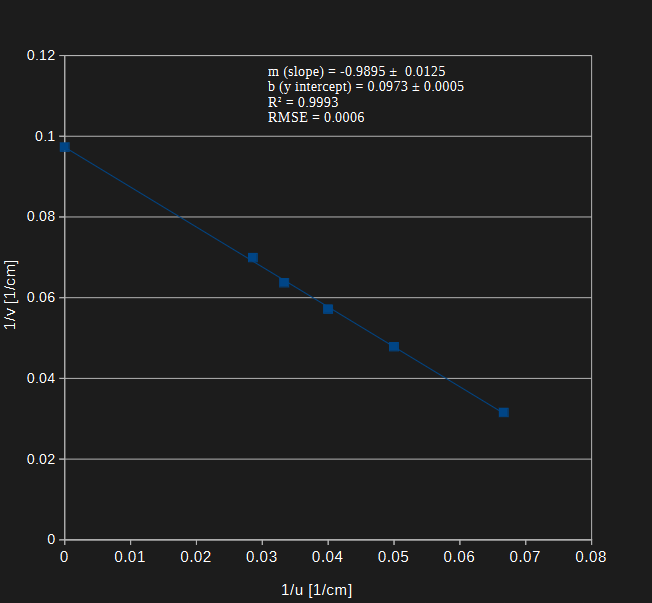
\includegraphics[width=0.8\textwidth]{Lab_1_Experiment_3.png}
  \caption{גרף המתאר את $1/u$ ו-$1/v$ כתלות זה בזה}
  \label{fig:excel_chart}
\end{figure}

על ידי העברת אגפים בחוק גאוס נקבל:
\begin{equation}
\frac{1}{v} = \frac{-1}{u} + \frac{1}{f}
\end{equation}

כלומר, החיתוך עם ציר ה-y בגרף הוא $\frac{1}{f}$, ומכאן נוכל למצוא את מרחק המוקד של העדשה המרכזת.
בעזרת רגרסיה ליניארית בכלי  בו ייצרנו  את הגרף מצאנו את y intercept, ששווה ל 0.0973
\begin{equation}
\frac{1}{f} = \frac{1}{0.0973} \Rightarrow f \approx 10.2775 cm \Rightarrow f \approx 102.775 mm
\end{equation}

\subsection*{דיון ומסקנות}
מרחק המוקד האמיתי של העדשה היה נתון בניסוי (כתוב על העדשה), וערכו היה 100 מ"מ.
השגיאה היחסית בין הערך שחישבנו לערך הידוע היא 2.775\%, ויכולה לנבוע מ:
\begin{itemize}
    \item חוסר דיוק במיקום המסך בעת קבלת הדמות
    \item שגיאת מדידה בסרגל על המסילה עליה התבצע הניסוי
\end{itemize}

בניסוי התבקשנו לבדוק האם ניתן למצוא דמות על המסך כאשר מניחים את העדשה במרחק קטן ממרחק המוקד מהעצם.
בעדשה מרכזת לא ניתן למצוא דמות על המסך במצב זה.

\section*{ניסוי 4 - מציאת מוקד עדשה מפזרת}
\subsection*{מטרת הניסוי}
מציאת מרחק המוקד של עדשה מפזרת
\subsection*{רקע תיאורטי}
עדשה מפזרת יוצרת דמות מדומה, הנוצרת כאשר קרני האור המתפזרות נראות כאילו הן מגיעות מנקודה מסוימת מאחורי העדשה. מרחק המוקד של עדשה מפזרת הוא תמיד מספר שלילי, כלומר $f < 0$.

\subsection*{מערכת המדידה ומהלך הניסוי}
הרכבנו על מסילה מקור אור, עדשה מרכזת, עדשה מפזרת ומסך (בסדר הזה), כך שנמצאת דמות על המסך.
המרחקים הם:
\begin{itemize}
    \item u1 - מרחק בין מקור האור לעדשה המרכזת = 21 ס"מ
    \item d - מרחק בין העדשה המרכזת לעדשה המפזרת = 11 ס"מ
    \item v2 - מרחק בין העדשה המפזרת למסך = 21.7 ס"מ
\end{itemize}

בעזרת נוסאת גאוס והערכים הללו נמצא את v1 - מרחק דמות הביניים הנורת בעדשה המרכזת מהעדשה. נשתמש במרחק המוקד של  העדשה המרכזת  אותו מצאנו בניסוי הקודם.

לאחר מכן נמצא u2 - מרחק גוף  הביניים מהעדשה המפזרת, וכך גם את מרחק המוקד של העדשה המפזרת - f2.

\subsection*{תוצאות וניתוח}
בינסוי הקודם מצאנו את מרחק המוקד של העדשה המרכזת, $f_1 = 102.775 mm$.
נחשב את מרחק דמות הביניים הנורת בעדשה המרכזת מהעדשה:

\begin{equation}
\begin{aligned}
\frac{1}{f_1} = \frac{1}{u_1} + \frac{1}{v_1}
\Rightarrow
\frac{1}{10.2775} = \frac{1}{21} + \frac{1}{v_1}
\Rightarrow
\\
\frac{1}{v_1} = \frac{1}{10.2775} - \frac{1}{21} \approx 0.047
\Rightarrow
v_1 \approx 20.13 cm
\end{aligned}
\end{equation}

ערכו של $v_1$ חיובי ולכן דמות הביניים מימין לעדשה המרכזת.

נחשב את $u2$ - מרחק גוף הביניים מהעדשה המפזרת, ואת $f_2$ - מרחק המוקד של העדשה המפזרת.
\begin{equation}
\begin{aligned}
u_2 = d - |v_1|
\Rightarrow
u_2 = 11 - 20.13 = -9.13 cm
\\
\frac{1}{f_2} = \frac{1}{u_2} + \frac{1}{v_2}
\Rightarrow
\frac{1}{f_2} = \frac{1}{-9.13} + \frac{1}{21.7}
\Rightarrow
f_2 \approx -15.76 cm
\end{aligned}
\end{equation}

\subsection*{דיון ומסקנות}
מרחק המוקד של העדשה המפזרת הוא מספר שלילי, כפי שצפינו.
הערך שחישבנו הוא 15.76- ס"מ, והערך הכתוב  על העדשה הוא -15 ס"מ.
השגיאה היחסית בין הערך שחישבנו לערך הידוע היא 5.07\%.

\end{document}